\documentclass[titlesec]{araproposal}

\usepackage{background}
\backgroundsetup{
  color=gray,
  opacity=0.2,
  contents=Preliminary
  }

% Examples
% Airborne Coronavirus Inactivation by Far-UVC Using a Coupled Radiation-CFD Model
% City Bus Cabin Air Monitoring and Conditioning for COVID19
% CFD Tool to Facilitate the Safe Re-Opening of Indoor Gyms
% Modelling of Air Distribution in Terraced Lecture Halls at the University of Waterloo
% Towards Safer Work Spaces: The Viability of Portable Air Purifiers

\hypersetup{
  pdftitle={ME663 - Computational Fluid Dynamics},
  pdfsubject={Proposal for research project},
  pdfauthor={Tommaso Bocchietti}
}

\title{Feasibility Investigation of Next-Generation Fuel Injectors using CFD Analysis}

\piauthor{Tommaso Bocchietti, Department of Mechanical \& Mechatronics Engineering, University of Waterloo}
% \copiauthorB{Co-PI Name, Title, Department Name, University Name}

\contact{Tommaso Bocchietti, \email{tbocchie@uwaterloo.ca}}
\date{\today}

\newcommand{\semph}[1]{\textbf{\textit{#1}}} % Strong emphasis
\newcommand{\para}[1]{\textbf{#1.}\ }

\begin{document}

\maketitle

\abstract{
  Nowadays, the importance of reducing emissions and increasing fuel efficiency has become even more crucial than ever.
  Some alternative technologies to traditional gasoline and diesel engines have been developed, such as electric vehicles or hydrogen fuel cells, but the transition to these new technologies is slow and expensive, and it is likely that internal combustion engines will be used for a long time to come.

  In this context, the development of new technologies that can be used in combination with existing engines structure is critical.
  The possibility of using alternative fuel sources, such as ammonia or dimethyl ether, is particularly attractive.
  These fuels have the potential to reduce emissions and increase fuel efficiency, but they require the development of new injectors that can handle their specific properties.

  In this research we will not focus on fuel engineering per se, but on the feasibility of a new generation of fuel injectors that can be fitted to existing engines and that can handle these alternative fuel sources.
  To do this, the use of Computational Fluid Dynamics (CFD) simulations will be critical, as it will allow us to study the interaction between fluid dynamics and the chemical reactions occurring within the injector in an efficient and cost-effective manner.
}

\keywords{Fuel injectors design, Computational Fluid Dynamics, Alternative fuel sources}

\section{Objectives and Impact}
\label{sec:objectives_and_impact}

\section{Background}
\label{sec:background}


\section{Research Plan and Methodology}
\label{sec:research_plan_and_methodology}

The research plan is divided into three main stages:

\begin{enumerate}
    \item Feasibility study: supposing that we will be able to design a fuel injector with no constraints, are those alternative fuels feasible to be used in internal combustion engines? What are their characteristics when it comes to ignite them under a controlled environment? $\rightarrow$ Understand the chemical and physical properties of the alternative fuels and their combustion process.
    \item Design and development of the fuel injector: based on the results of the feasibility study, modelling and simulation of diverse fuel injectors designs. $\rightarrow$ Use CFD simulations to optimize the fuel injector design.
    \item Experimental validation: once the simulations are completed, we will build a prototype and test it in a controlled environment. $\rightarrow$ Compare the experimental results with the simulations. Eventually, rerun CFD simulations to improve the model (and the design).
\end{enumerate}
\section{Preliminary Results}
\label{sec:preliminary_results}

A preliminary result would be about a rough estimation of a possible design of the fuel injector.

This implies to have a deep understanding of the chemical and physical properties of the alternative fuels and their combustion process.
Given that we don't have such a background in chemistry, nor we have the capability to perform a real CFD simulation, we can only try to replicate the results of the current state of the art just to have a starting point for our research.

\begin{figure}[H]
    \centering
    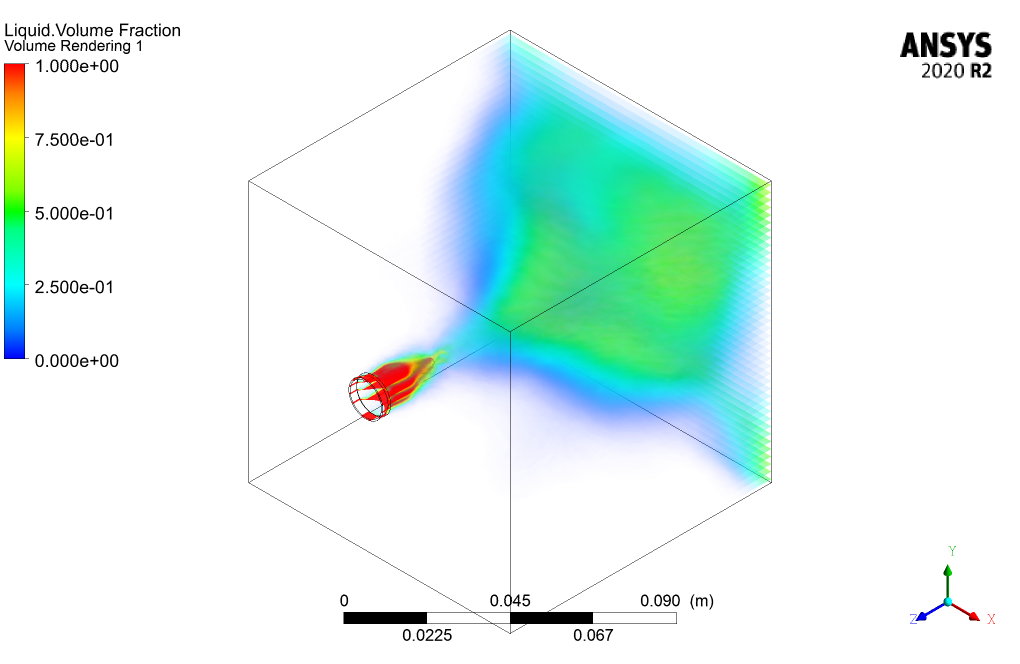
\includegraphics[width=0.8\textwidth]{img/injector_analysis_example.png}
    \caption{\href{https://www.mr-cfd.com/shop/fuel-injector-cfd-simulation-three-phase-flow/}{Analysis of a generic fuel injector.}}
    \label{fig:fuel_injector_analysis}
\end{figure}
\section{Deliverables}
\label{sec:deliverables}

The deliverables of this research project are:

\begin{itemize}
    \item A feasibility study of the use of alternative fuels in current internal combustion engines.
    \item A new fuel injector design that can handle alternative fuels.
    \item A set of models and simulations that can be used to optimize the fuel injector design.
\end{itemize}

\appendix

% \newpage
% \cite{ara}
% \bibliographystyle{plainurl}
% \bibliography{ref}

\end{document}


